\documentclass[12pt,a4paper]{article}

% Essential packages
\usepackage[utf8]{inputenc}
\usepackage[T1]{fontenc}
\usepackage{amsmath,amssymb,amsfonts}
\usepackage{graphicx}
\usepackage{float}
\usepackage[margin=1in]{geometry}
\usepackage{hyperref}
\usepackage{fancyhdr}
\usepackage{tikz}
\usepackage{pgfplots}
\pgfplotsset{compat=1.17}
\usepackage{tcolorbox}
\usepackage{booktabs}
\usepackage{enumitem}
\usepackage{xcolor}

% Fix header height
\setlength{\headheight}{14.5pt}

% Color definitions
\definecolor{conceptblue}{RGB}{230,240,255}
\definecolor{exampleorange}{RGB}{255,245,230}
\definecolor{importantred}{RGB}{255,235,235}
\definecolor{deepgreen}{RGB}{220,245,220}
\definecolor{mathpurple}{RGB}{245,235,255}

% Custom environments
\newtcolorbox{conceptbox}[1][]{
    colback=conceptblue,
    colframe=blue!60!black,
    title=#1,
    fonttitle=\bfseries,
    boxrule=0.5pt,
    arc=3pt
}

\newtcolorbox{examplebox}[1][]{
    colback=exampleorange,
    colframe=orange!80!black,
    title=#1,
    fonttitle=\bfseries,
    boxrule=0.5pt,
    arc=3pt
}

\newtcolorbox{importantbox}{
    colback=importantred,
    colframe=red!70!black,
    boxrule=0.5pt,
    arc=3pt
}

\newtcolorbox{deepexplanation}{
    colback=deepgreen,
    colframe=green!50!black,
    boxrule=1pt,
    arc=4pt,
    left=8pt,
    right=8pt,
    top=8pt,
    bottom=8pt
}

\newtcolorbox{mathbox}{
    colback=mathpurple,
    colframe=purple!60!black,
    boxrule=0.5pt,
    arc=3pt
}

% Header/Footer
\pagestyle{fancy}
\fancyhf{}
\fancyhead[L]{Chapter 5: Image Restoration and Reconstruction}
\fancyhead[R]{Digital Image Processing}
\fancyfoot[C]{\thepage}

\title{\textbf{Chapter 5: Image Restoration and Reconstruction}\\
\Large Comprehensive Study Notes with Deep Technical Analysis\\
\normalsize Based on Gonzalez \& Woods (3rd Edition) and CPE415 Lecture 12}
\author{Study Notes with Deep Technical Explanations}
\date{Spring 2026}

\begin{document}

\maketitle
\tableofcontents
\newpage

%==============================================================================
\section{Introduction: Enhancement vs. Restoration}
%==============================================================================

\begin{conceptbox}[Core Idea of Restoration]
\textbf{Image enhancement} improves visual appearance, often without an explicit degradation model.

\textbf{Image restoration} uses a mathematical model of degradation and noise to recover an estimate of the original image.

The standard model is:
\[
g(x,y) = H[f(x,y)] + \eta(x,y)
\]
where:
\begin{itemize}
    \item $f(x,y)$ = original image
    \item $H$ = degradation operator (blur, motion, turbulence, etc.)
    \item $\eta(x,y)$ = additive noise
    \item $g(x,y)$ = observed degraded image
\end{itemize}
\end{conceptbox}

In frequency domain (for linear, position-invariant degradation), the same model becomes:
\[
G(u,v) = H(u,v)F(u,v) + N(u,v)
\]
This is the central equation of Chapter 5.

\begin{deepexplanation}
\textbf{DEEP ANALYSIS: Why Chapter 5 Matters}

Chapter 4 taught us how to filter in frequency domain. Chapter 5 now uses that foundation to solve a harder problem:
\begin{itemize}
    \item Not only to smooth or sharpen,
    \item but to \textbf{undo known distortions} caused by physical acquisition systems.
\end{itemize}

The challenge is that inversion is numerically unstable:
\begin{itemize}
    \item If $H(u,v)$ is small, dividing by it amplifies noise.
    \item So restoration is always a tradeoff between deblurring and noise amplification.
\end{itemize}
\end{deepexplanation}

%==============================================================================
\section{Periodic Noise Reduction in Frequency Domain}
%==============================================================================

\subsection{Bandreject and Notch Filtering}

Periodic interference creates localized spikes in the Fourier spectrum. Instead of using broad LPF/HPF operations, we can remove only selected frequencies:

\begin{itemize}
    \item \textbf{Bandreject filter}: suppresses a circular/ring-like frequency band.
    \item \textbf{Notch reject filter}: suppresses small neighborhoods around specific frequency locations.
\end{itemize}

For corresponding notch-pass and notch-reject filters:
\[
H_{NP}(u,v) = 1 - H_{NR}(u,v)
\]

\begin{figure}[H]
    \centering
    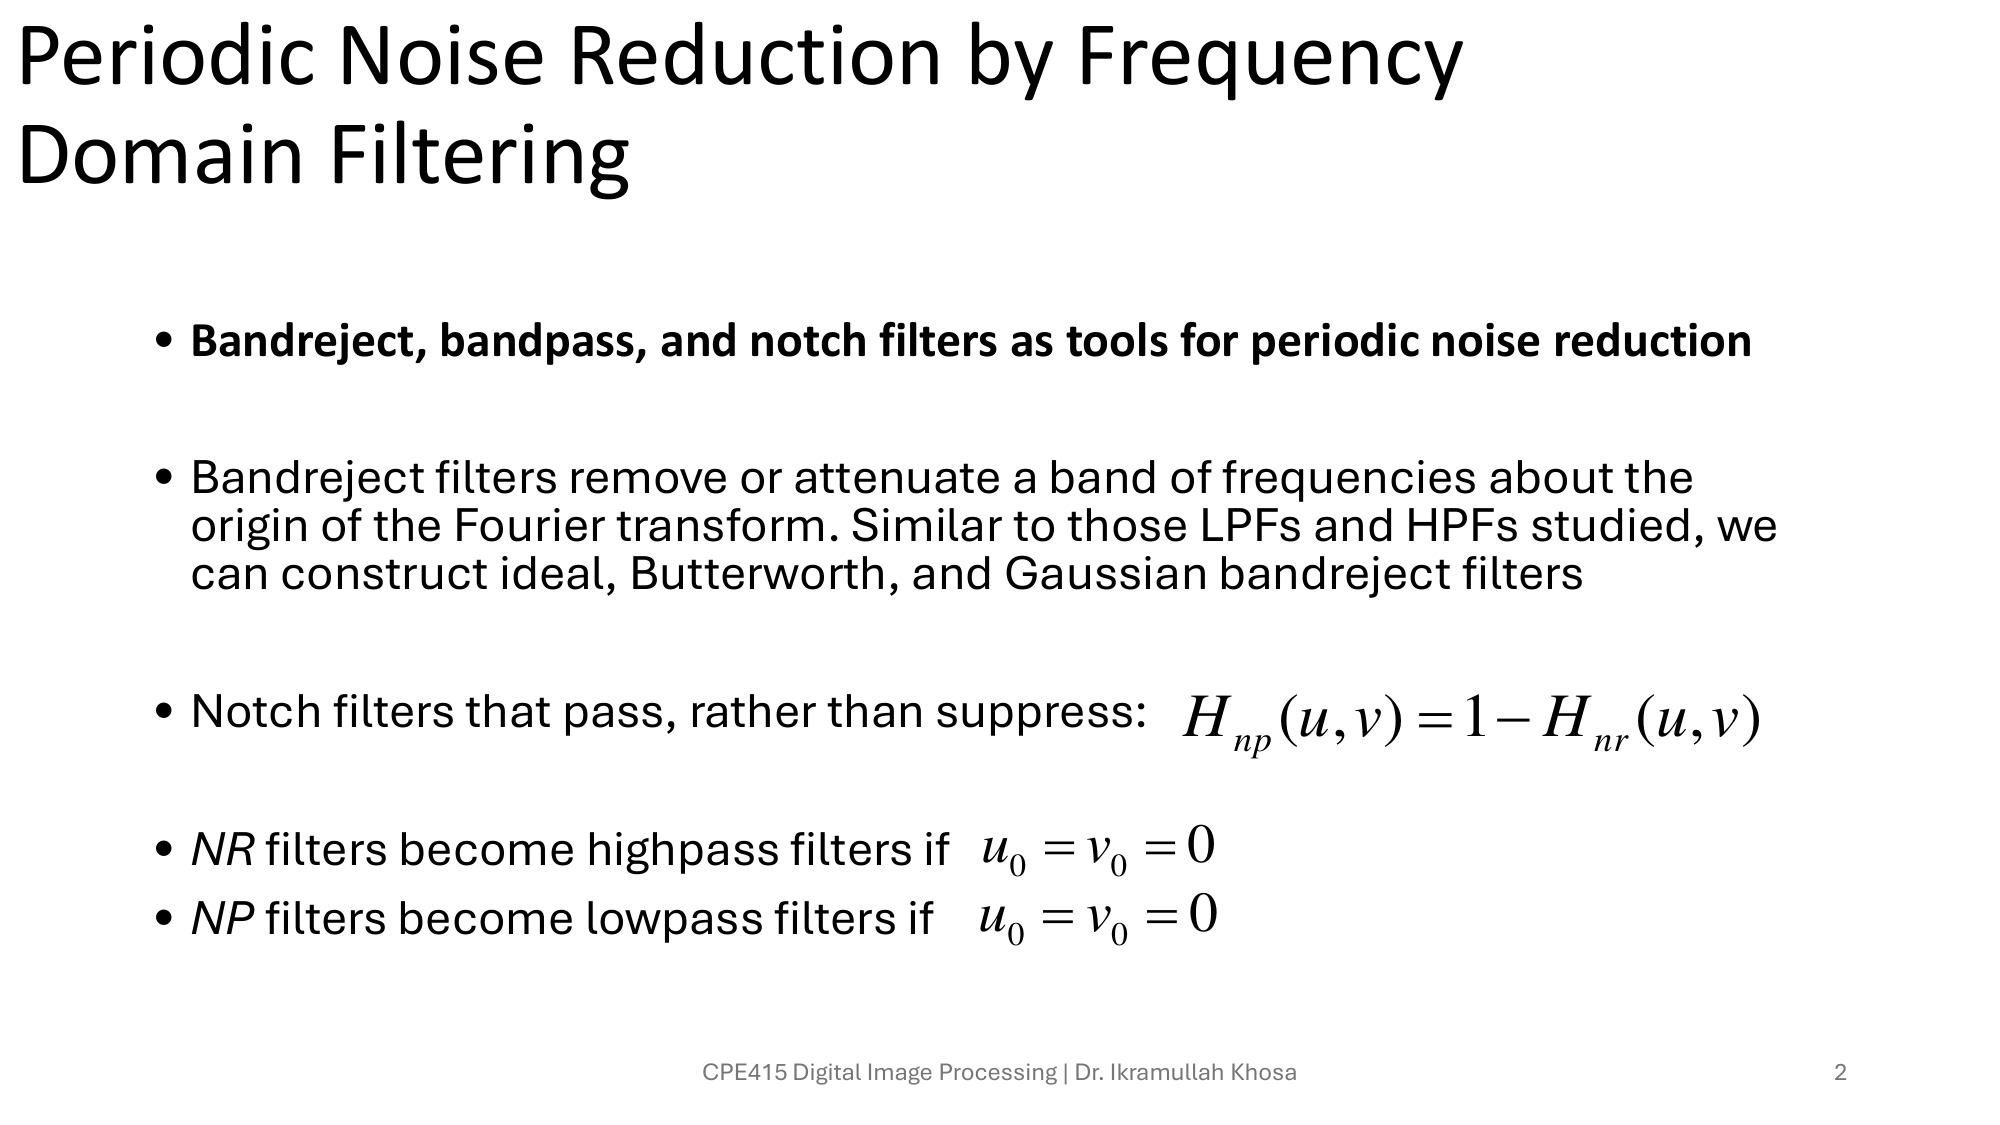
\includegraphics[width=0.9\textwidth]{images/slide12-02.png}
    \caption{Lecture 12 overview of periodic noise reduction with bandreject/notch concepts}
    \label{fig:periodic_overview}
\end{figure}

\begin{figure}[H]
    \centering
    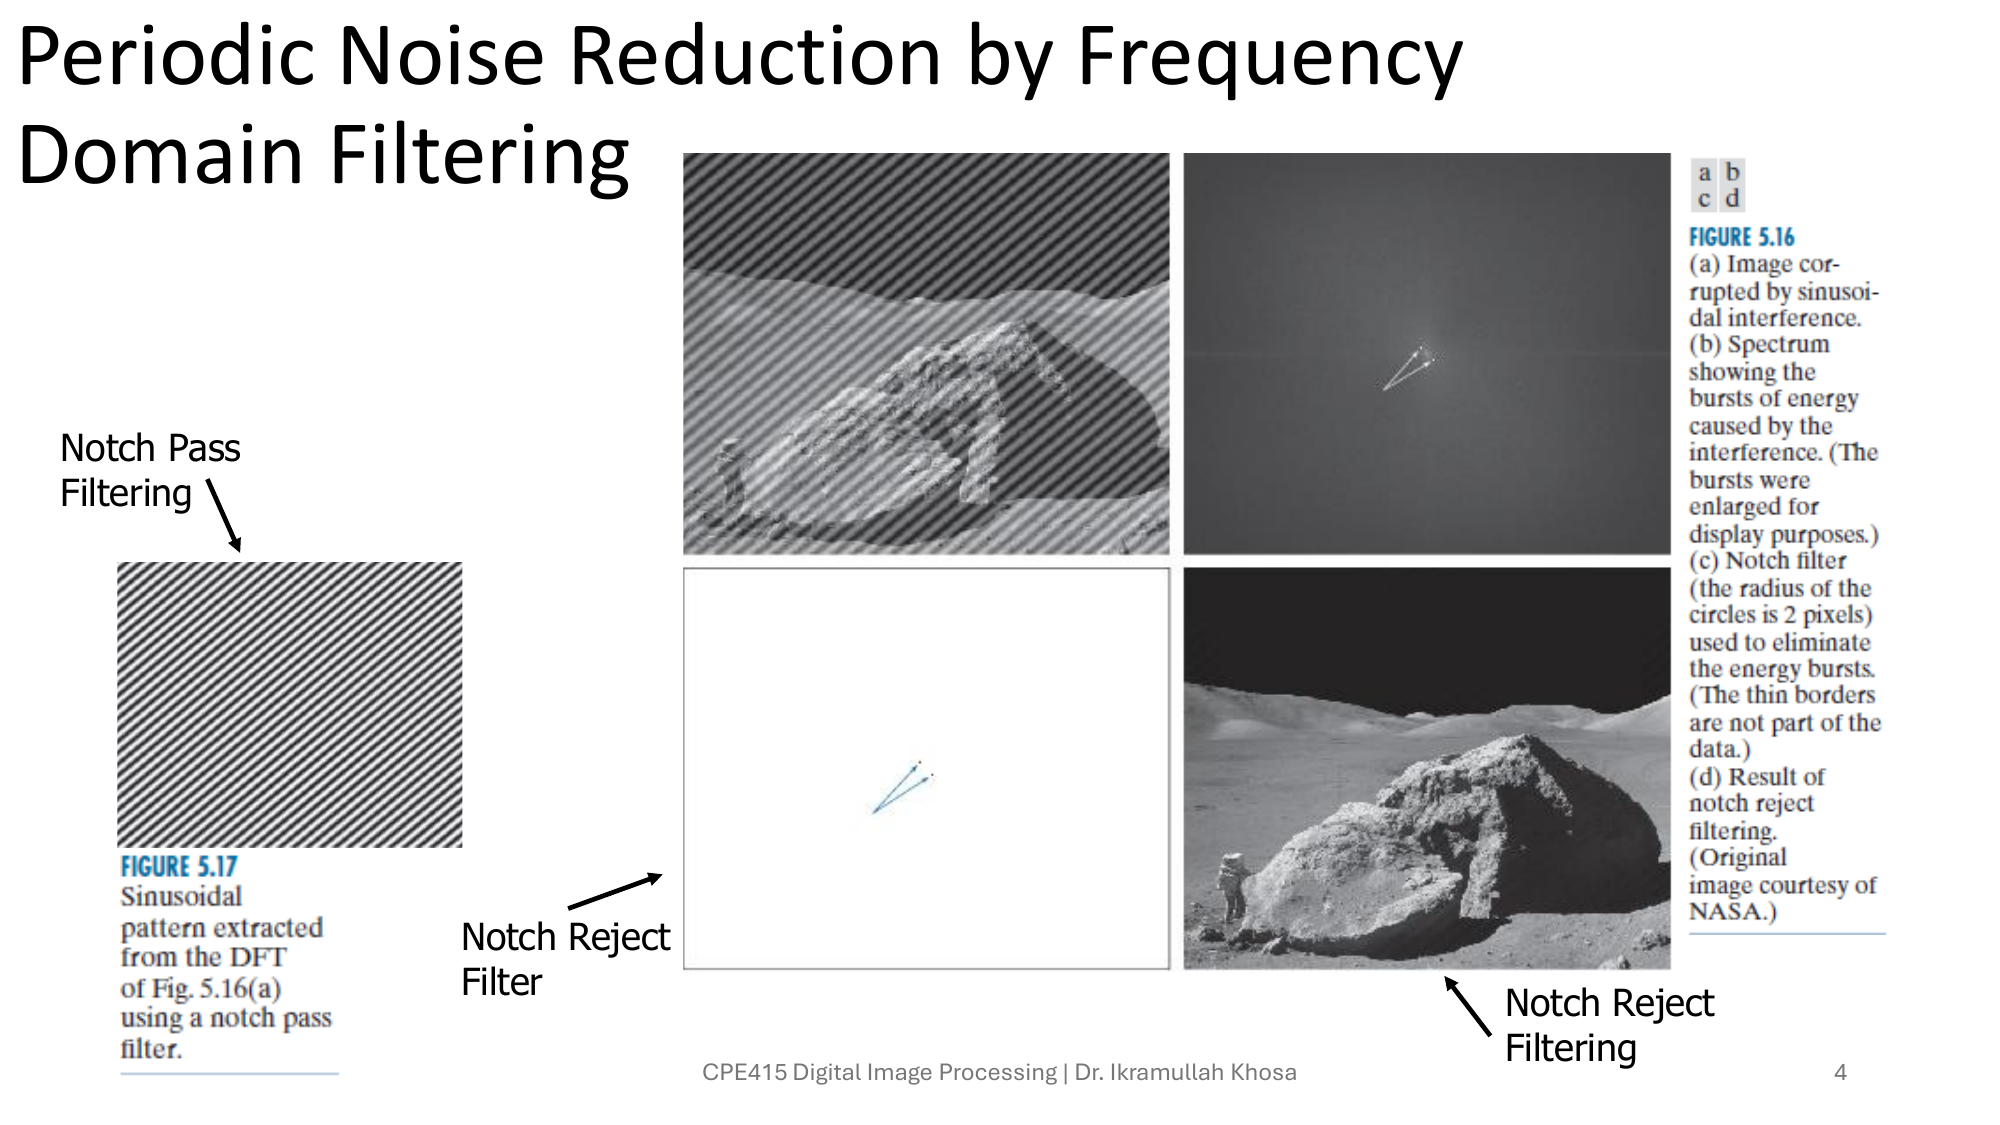
\includegraphics[width=0.9\textwidth]{images/slide12-04.png}
    \caption{Notch pass and notch reject filtering examples}
    \label{fig:notch_examples}
\end{figure}

\begin{deepexplanation}
\textbf{DEEP ANALYSIS - Notch Filtering Strategy}

Practical steps:
\begin{enumerate}
    \item Compute centered FFT of degraded image.
    \item Locate periodic-noise spikes (always consider conjugate-symmetric pairs).
    \item Build notch-pass mask to isolate noise pattern.
    \item Convert to notch-reject mask and apply to $G(u,v)$.
    \item Inverse FFT to obtain cleaned image.
\end{enumerate}

Why not always use LPF?
\begin{itemize}
    \item LPF removes high-frequency noise \textbf{and} fine detail.
    \item Notch filtering is selective and preserves more image information.
\end{itemize}
\end{deepexplanation}

\subsection{Optimum Notch Filtering}

If extracted interference pattern is only an approximation, direct subtraction is suboptimal.
Use weighted subtraction:
\[
\hat{f}(x,y) = g(x,y) - w(x,y)\hat{\eta}(x,y)
\]
where $w(x,y)$ is chosen to minimize local variance in a neighborhood.

A local variance form is:
\[
\sigma^2(x,y)=\frac{1}{(2a+1)(2b+1)}\sum_{s=-a}^{a}\sum_{t=-b}^{b}\left[\hat{f}(x+s,y+t)-\overline{\hat{f}}(x,y)\right]^2
\]

Optimizing gives a closed form (from chapter derivation):
\[
w(x,y) = \frac{\overline{g\hat{\eta}}-\overline{g}\,\overline{\hat{\eta}}}{\overline{\hat{\eta}^2}-\left(\overline{\hat{\eta}}\right)^2}
\]
(Equivalent local-statistics form; bars denote neighborhood averages.)

\begin{figure}[H]
    \centering
    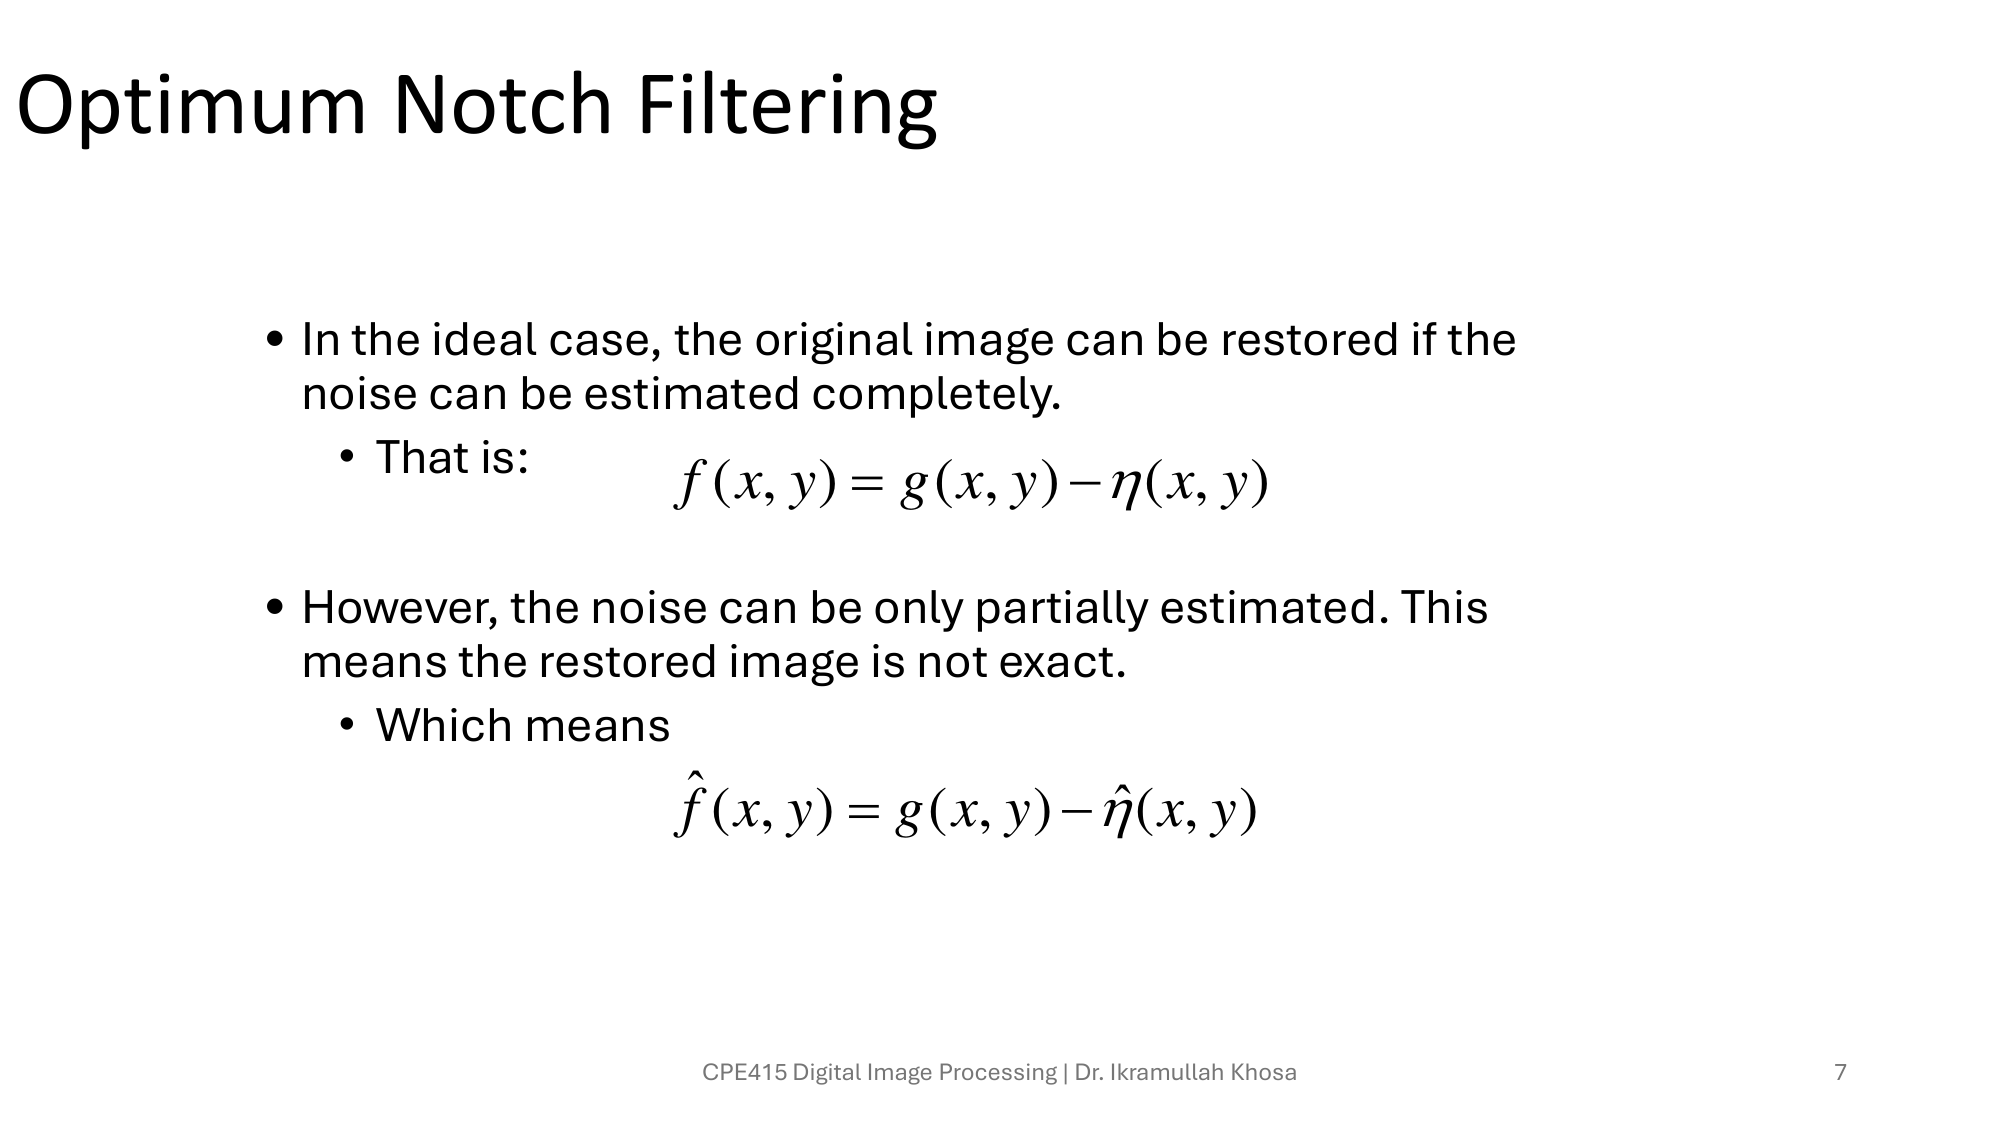
\includegraphics[width=0.85\textwidth]{images/slide12-07.png}
    \caption{Optimum notch filtering formulation from lecture}
    \label{fig:opt_notch_1}
\end{figure}

\begin{figure}[H]
    \centering
    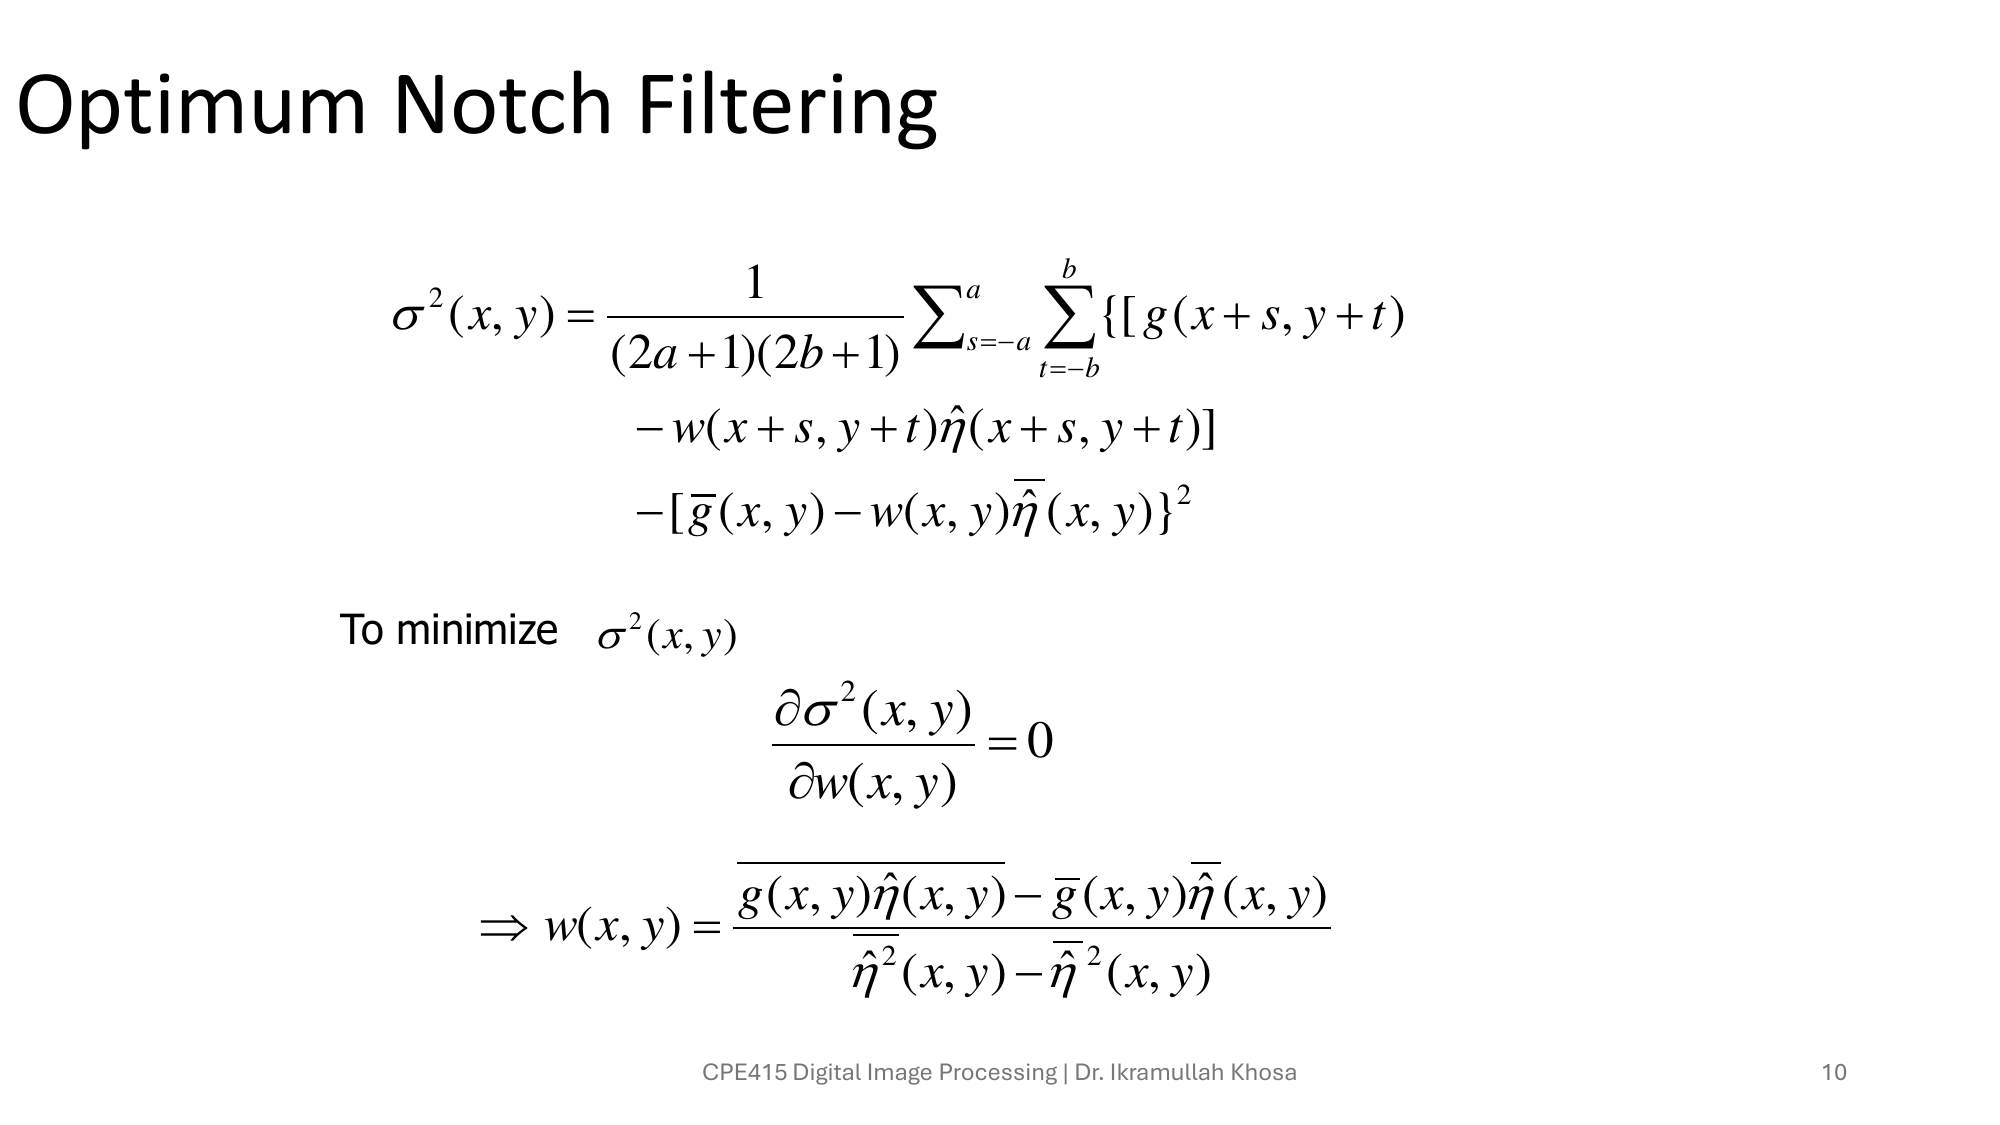
\includegraphics[width=0.85\textwidth]{images/slide12-10.png}
    \caption{Local-variance minimization leading to optimum modulation function}
    \label{fig:opt_notch_2}
\end{figure}

%==============================================================================
\section{Linear, Position-Invariant Degradation Model}
%==============================================================================

For linear, shift-invariant systems:
\[
g(x,y)=h(x,y) * f(x,y) + \eta(x,y)
\]
and in frequency domain:
\[
G(u,v)=H(u,v)F(u,v)+N(u,v)
\]

\begin{conceptbox}[Why LSI Model Is So Important]
The LSI assumption makes restoration tractable:
\begin{itemize}
    \item Convolution in spatial domain becomes multiplication in frequency domain.
    \item Powerful tools from linear systems theory become usable.
    \item Many practical degradations (defocus blur, mild turbulence, motion blur) are approximated well enough by LSI.
\end{itemize}
\end{conceptbox}

%==============================================================================
\section{Estimating the Degradation Function $H(u,v)$}
%==============================================================================

There are three principal approaches:
\begin{enumerate}
    \item \textbf{Observation from degraded image}
    \item \textbf{Experimentation} (impulse response measurement)
    \item \textbf{Mathematical modeling}
\end{enumerate}

\subsection{Estimation by Observation}
Choose a high-contrast subimage $g_s(x,y)$ and construct a sharpened estimate $\hat{f}_s(x,y)$.
Then:
\[
H_s(u,v) = \frac{G_s(u,v)}{\hat{F}_s(u,v)}
\]
Infer full $H(u,v)$ shape from this estimate.

\subsection{Estimation by Experimentation}
Image a near-impulse (small bright point) using same system settings. If impulse has strength $A$:
\[
H(u,v)=\frac{G(u,v)}{A}
\]

\subsection{Estimation by Modeling}

\textbf{Atmospheric turbulence model:}
\[
H(u,v)=e^{-k(u^2+v^2)^{5/6}}
\]
where $k$ controls turbulence severity.

\begin{figure}[H]
    \centering
    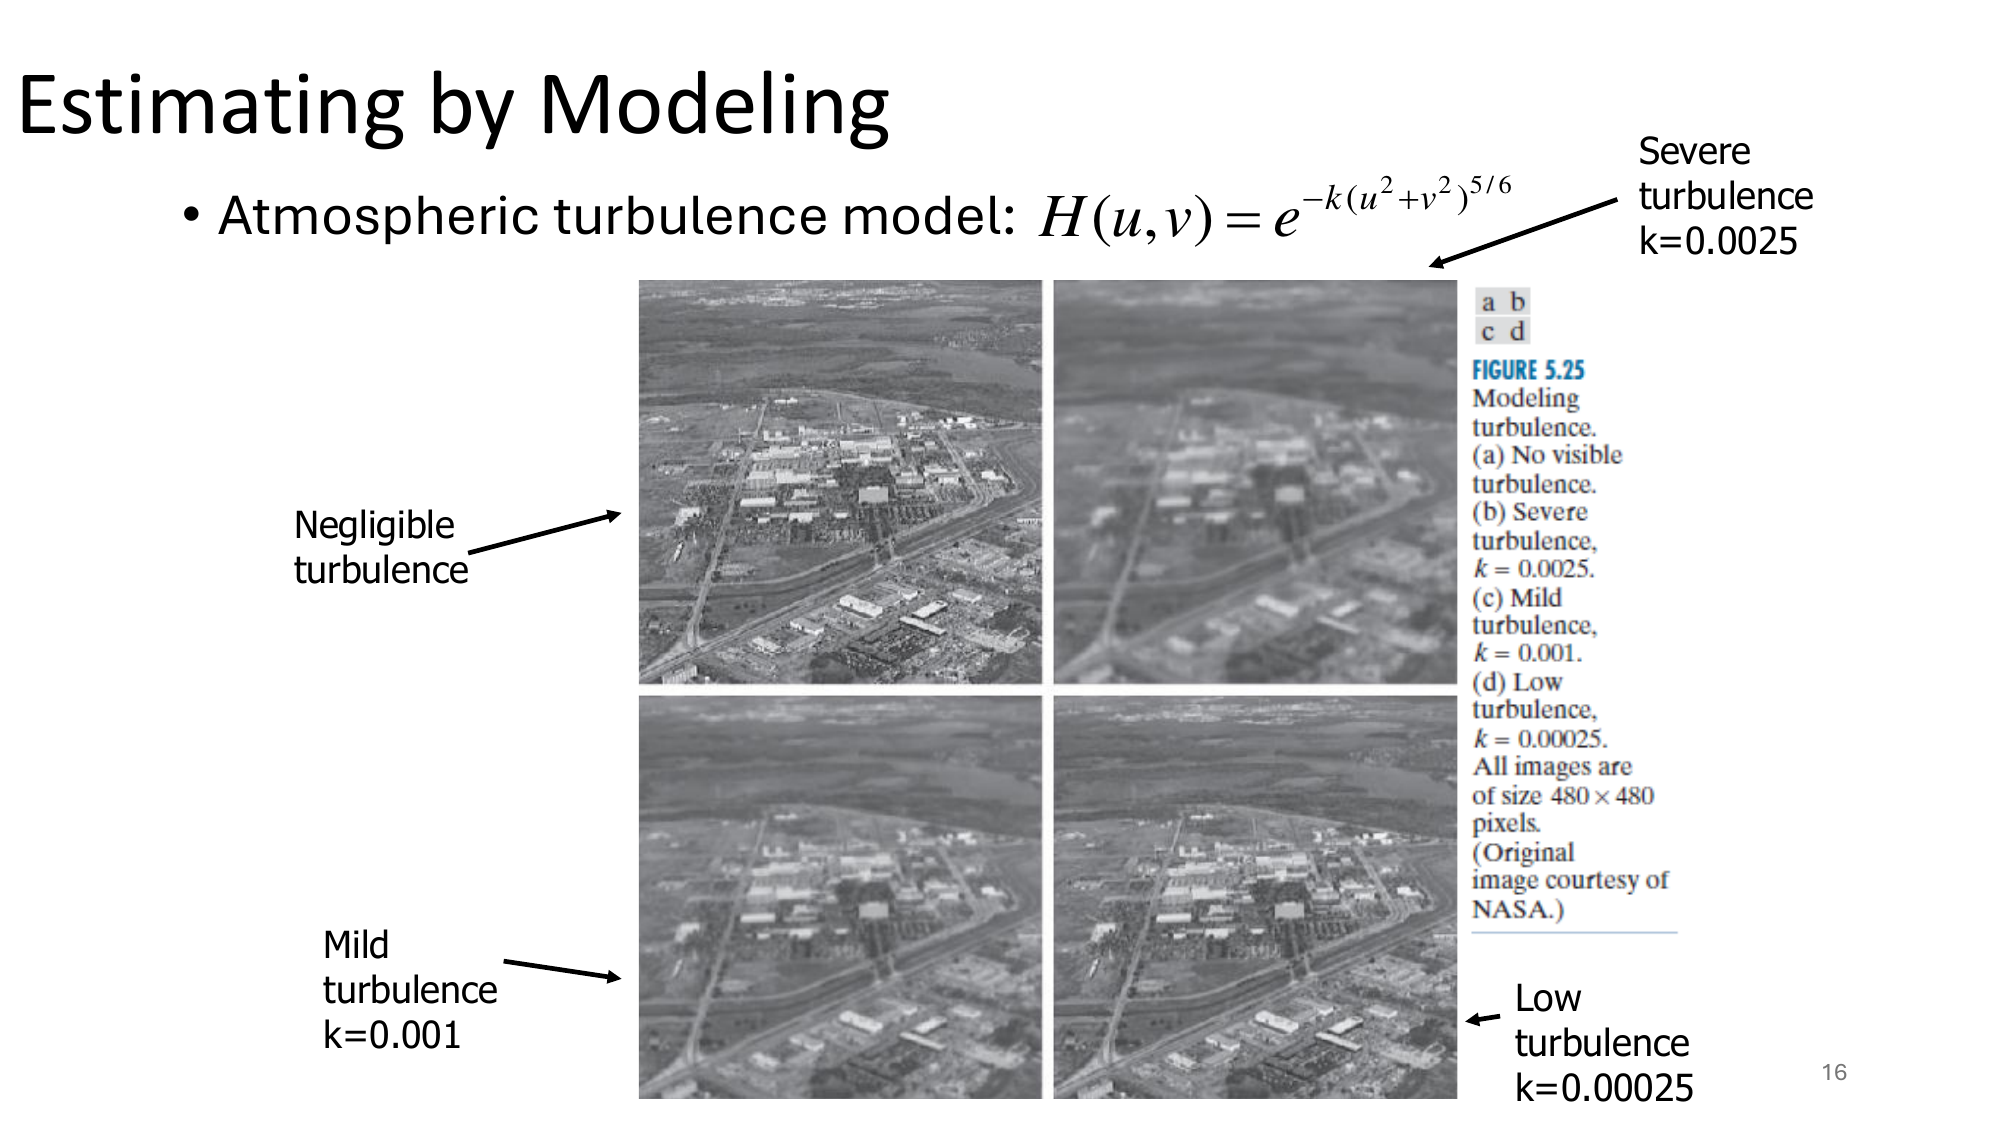
\includegraphics[width=0.85\textwidth]{images/slide12-16.png}
    \caption{Model-based estimation example: atmospheric turbulence}
    \label{fig:turbulence}
\end{figure}

\textbf{Uniform linear motion blur:}
\[
g(x,y)=\int_0^T f[x-x_0(t),\,y-y_0(t)]\,dt
\]
For $x_0(t)=at/T$ and $y_0(t)=bt/T$, degradation in frequency domain becomes:
\[
H(u,v)=\frac{T}{\pi(ua+vb)}\sin\left[\pi(ua+vb)\right]e^{-j\pi(ua+vb)}
\]

\begin{figure}[H]
    \centering
    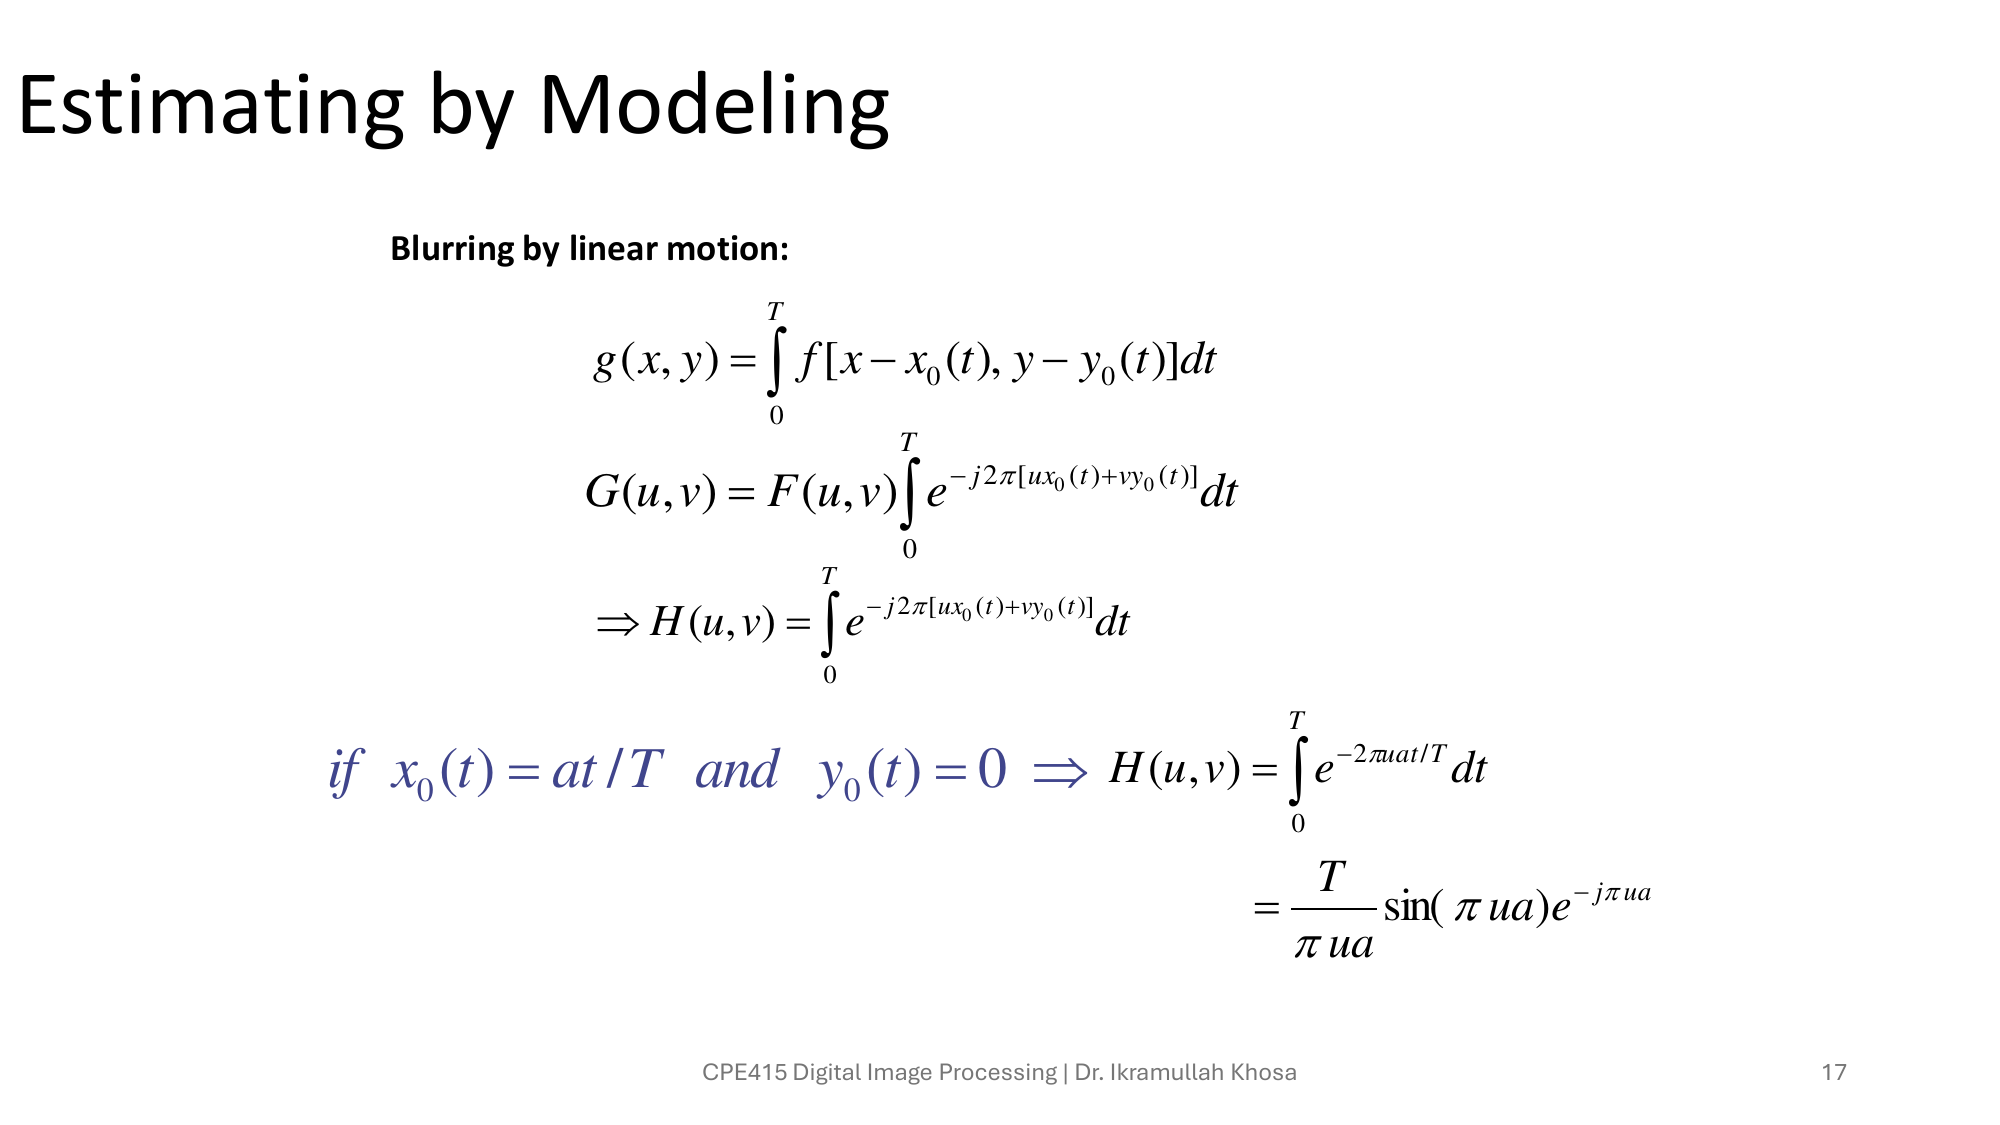
\includegraphics[width=0.85\textwidth]{images/slide12-17.png}
    \caption{Linear motion blur derivation (special case and sinc form)}
    \label{fig:motion_model_1}
\end{figure}

\begin{figure}[H]
    \centering
    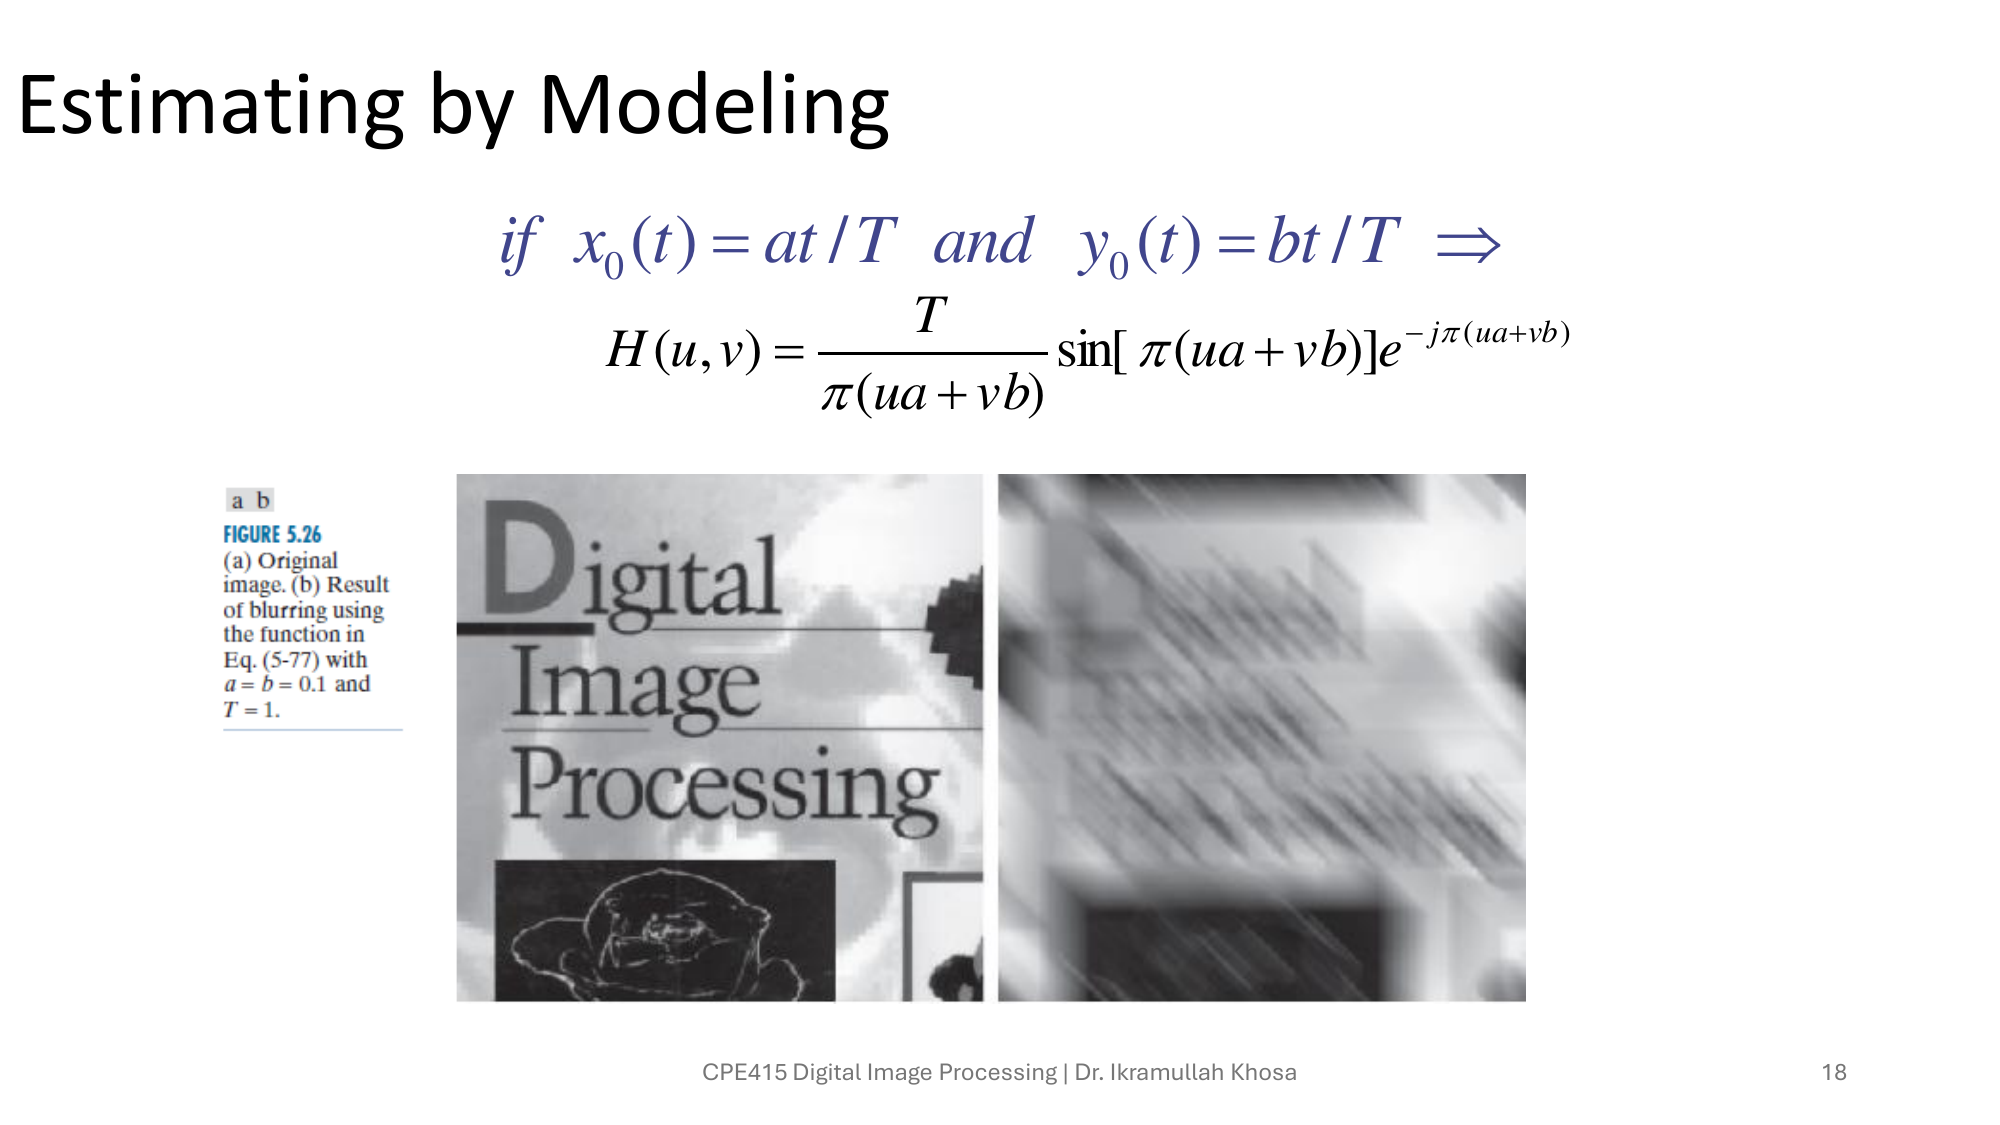
\includegraphics[width=0.85\textwidth]{images/slide12-18.png}
    \caption{General linear motion blur model with both x and y motion}
    \label{fig:motion_model_2}
\end{figure}

%==============================================================================
\section{Inverse Filtering}
%==============================================================================

The most direct restoration method is:
\[
\hat{F}(u,v)=\frac{G(u,v)}{H(u,v)}
\]
Substituting degradation model gives:
\[
\hat{F}(u,v)=F(u,v)+\frac{N(u,v)}{H(u,v)}
\]

\begin{importantbox}
\textbf{Critical Limitation:}
If $H(u,v)$ has zeros or very small values, $N(u,v)/H(u,v)$ explodes and dominates the estimate.
So direct inverse filtering is usually unstable in the presence of noise.
\end{importantbox}

A practical fix is radial limitation (lowpass-limited inverse filtering), where inverse operation is applied only near origin where $|H(u,v)|$ is larger.

\begin{figure}[H]
    \centering
    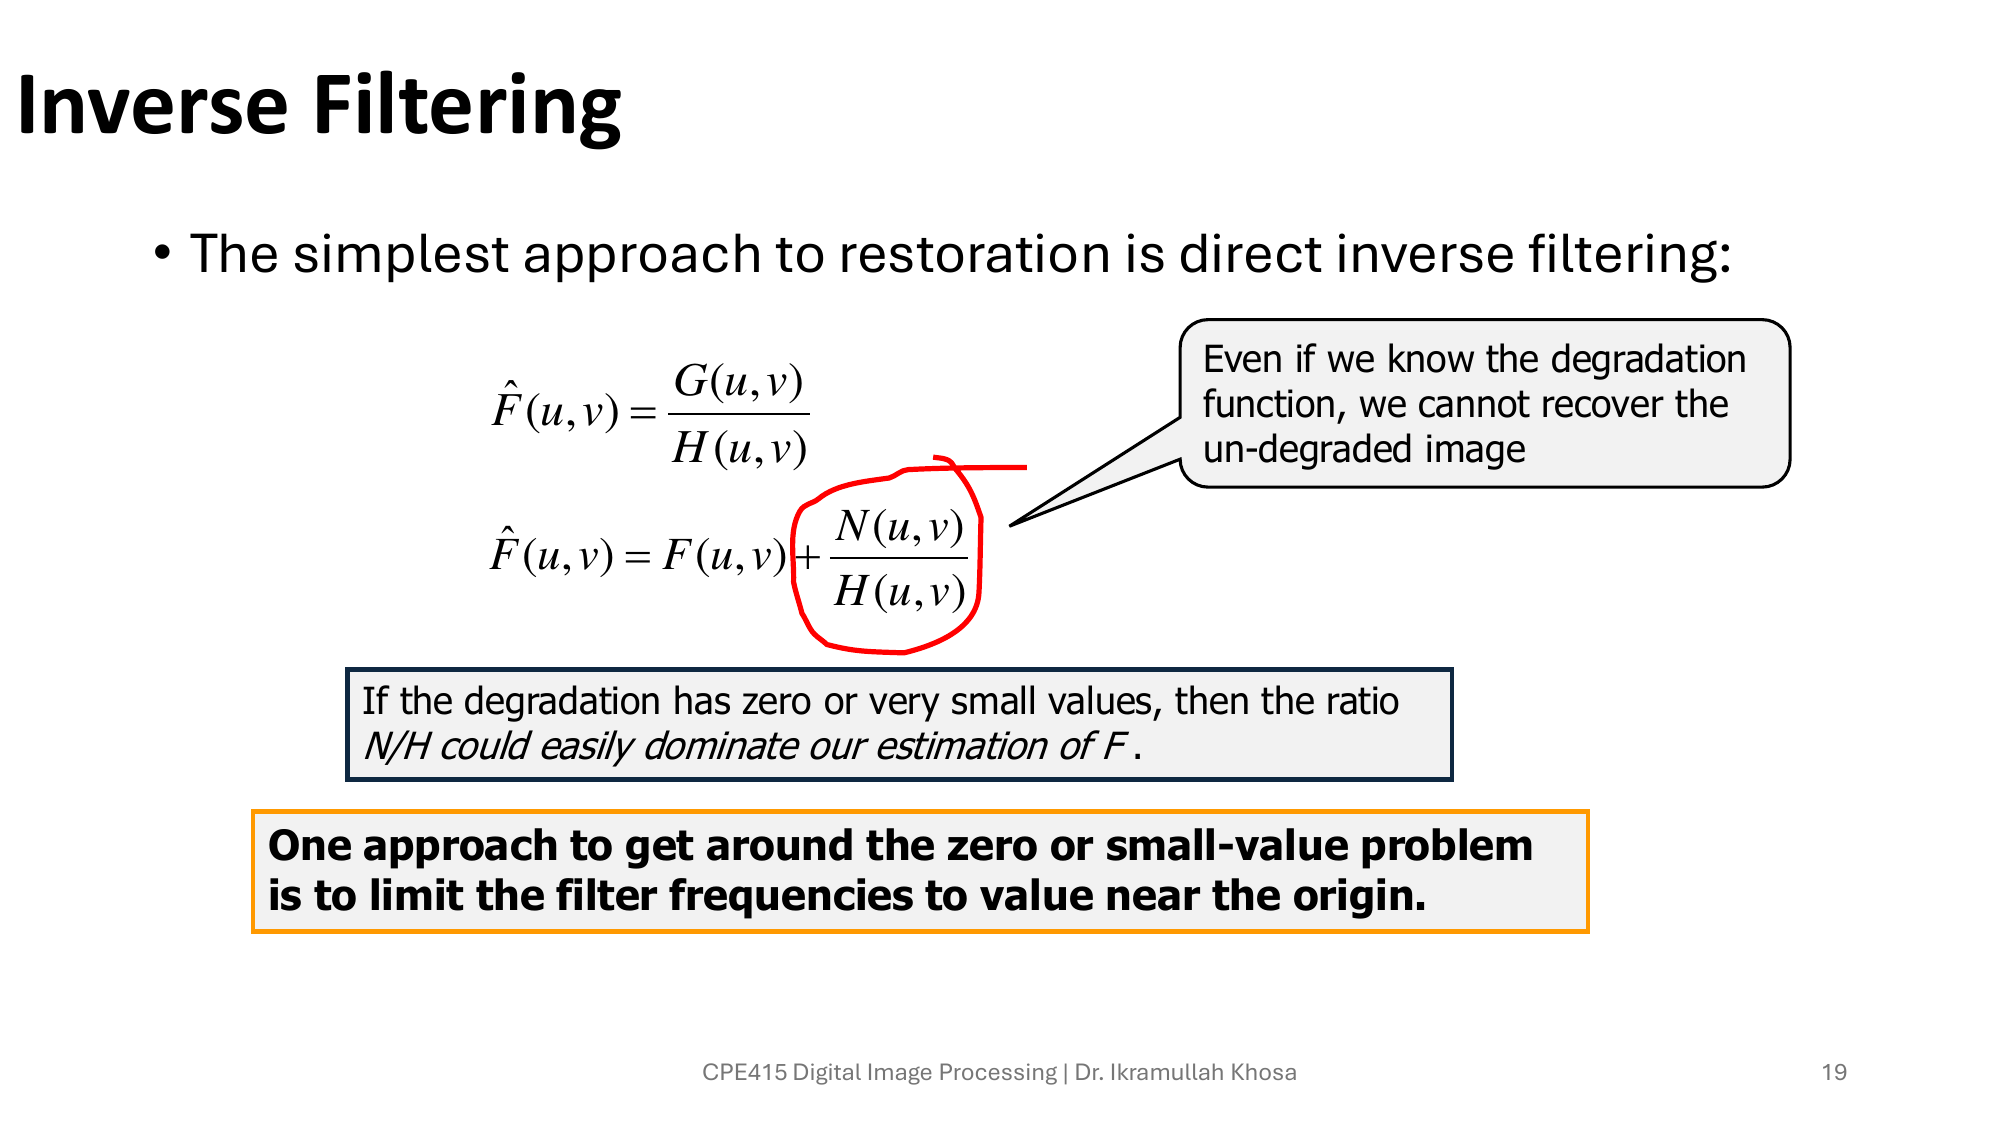
\includegraphics[width=0.9\textwidth]{images/slide12-19.png}
    \caption{Inverse filtering and noise-amplification issue from Lecture 12}
    \label{fig:inverse_filtering}
\end{figure}

\begin{figure}[H]
    \centering
    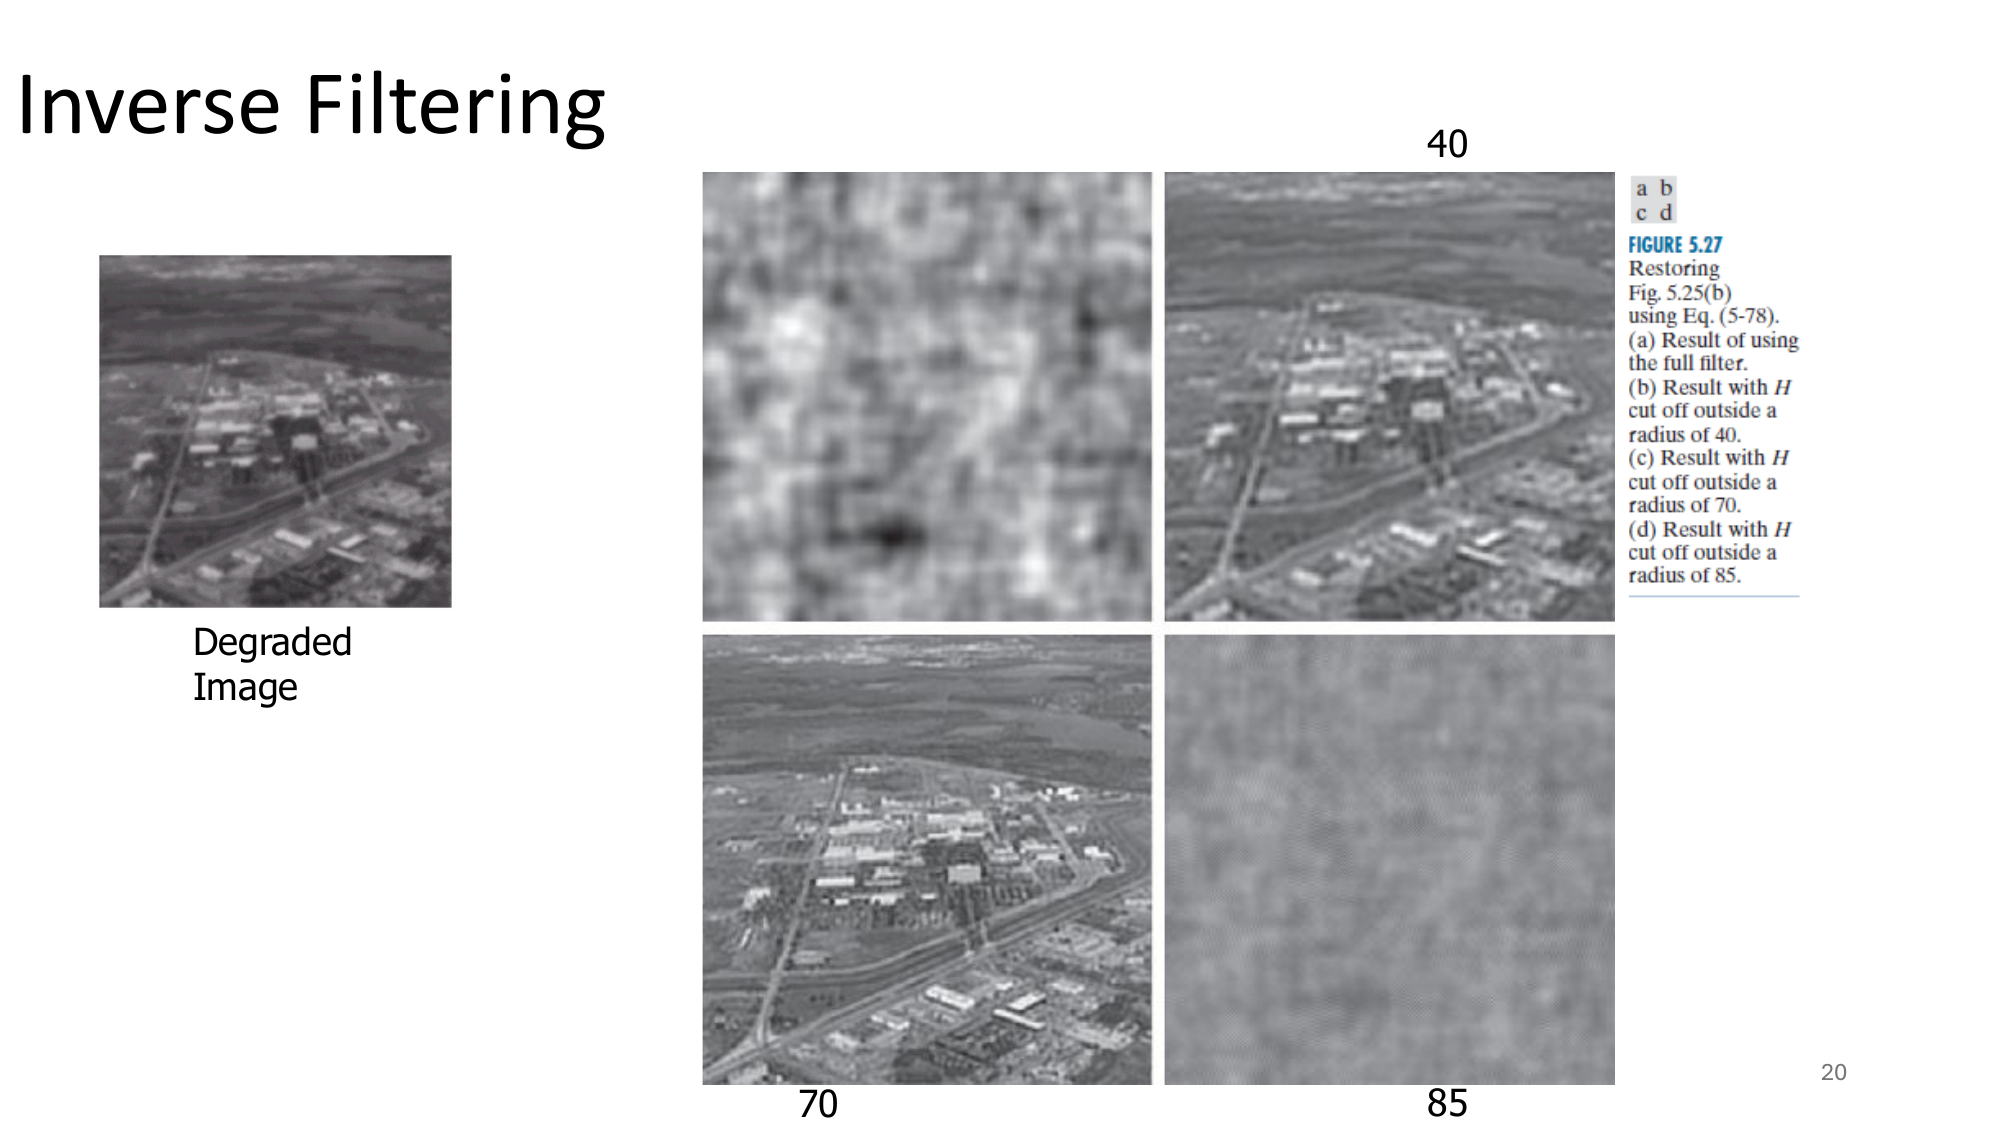
\includegraphics[width=0.9\textwidth]{images/slide12-20.png}
    \caption{Example of radius-limited inverse restoration}
    \label{fig:inverse_radius}
\end{figure}

%==============================================================================
\section{Minimum Mean Square Error (Wiener) Filtering}
%==============================================================================

Wiener filtering minimizes mean square error:
\[
e^2 = E\left[(f-\hat{f})^2\right]
\]

Frequency-domain Wiener estimate:
\[
\hat{F}(u,v)=\left[\frac{H^*(u,v)}{|H(u,v)|^2+\frac{S_\eta(u,v)}{S_f(u,v)}}\right]G(u,v)
\]
where:
\begin{itemize}
    \item $H^*(u,v)$ is complex conjugate of $H(u,v)$,
    \item $S_\eta(u,v)$ is noise power spectrum,
    \item $S_f(u,v)$ is original-image power spectrum.
\end{itemize}

Common practical approximation:
\[
\hat{F}(u,v)=\left[\frac{H^*(u,v)}{|H(u,v)|^2+K}\right]G(u,v)
\]
with $K$ as a constant approximation to $S_\eta/S_f$.

\begin{figure}[H]
    \centering
    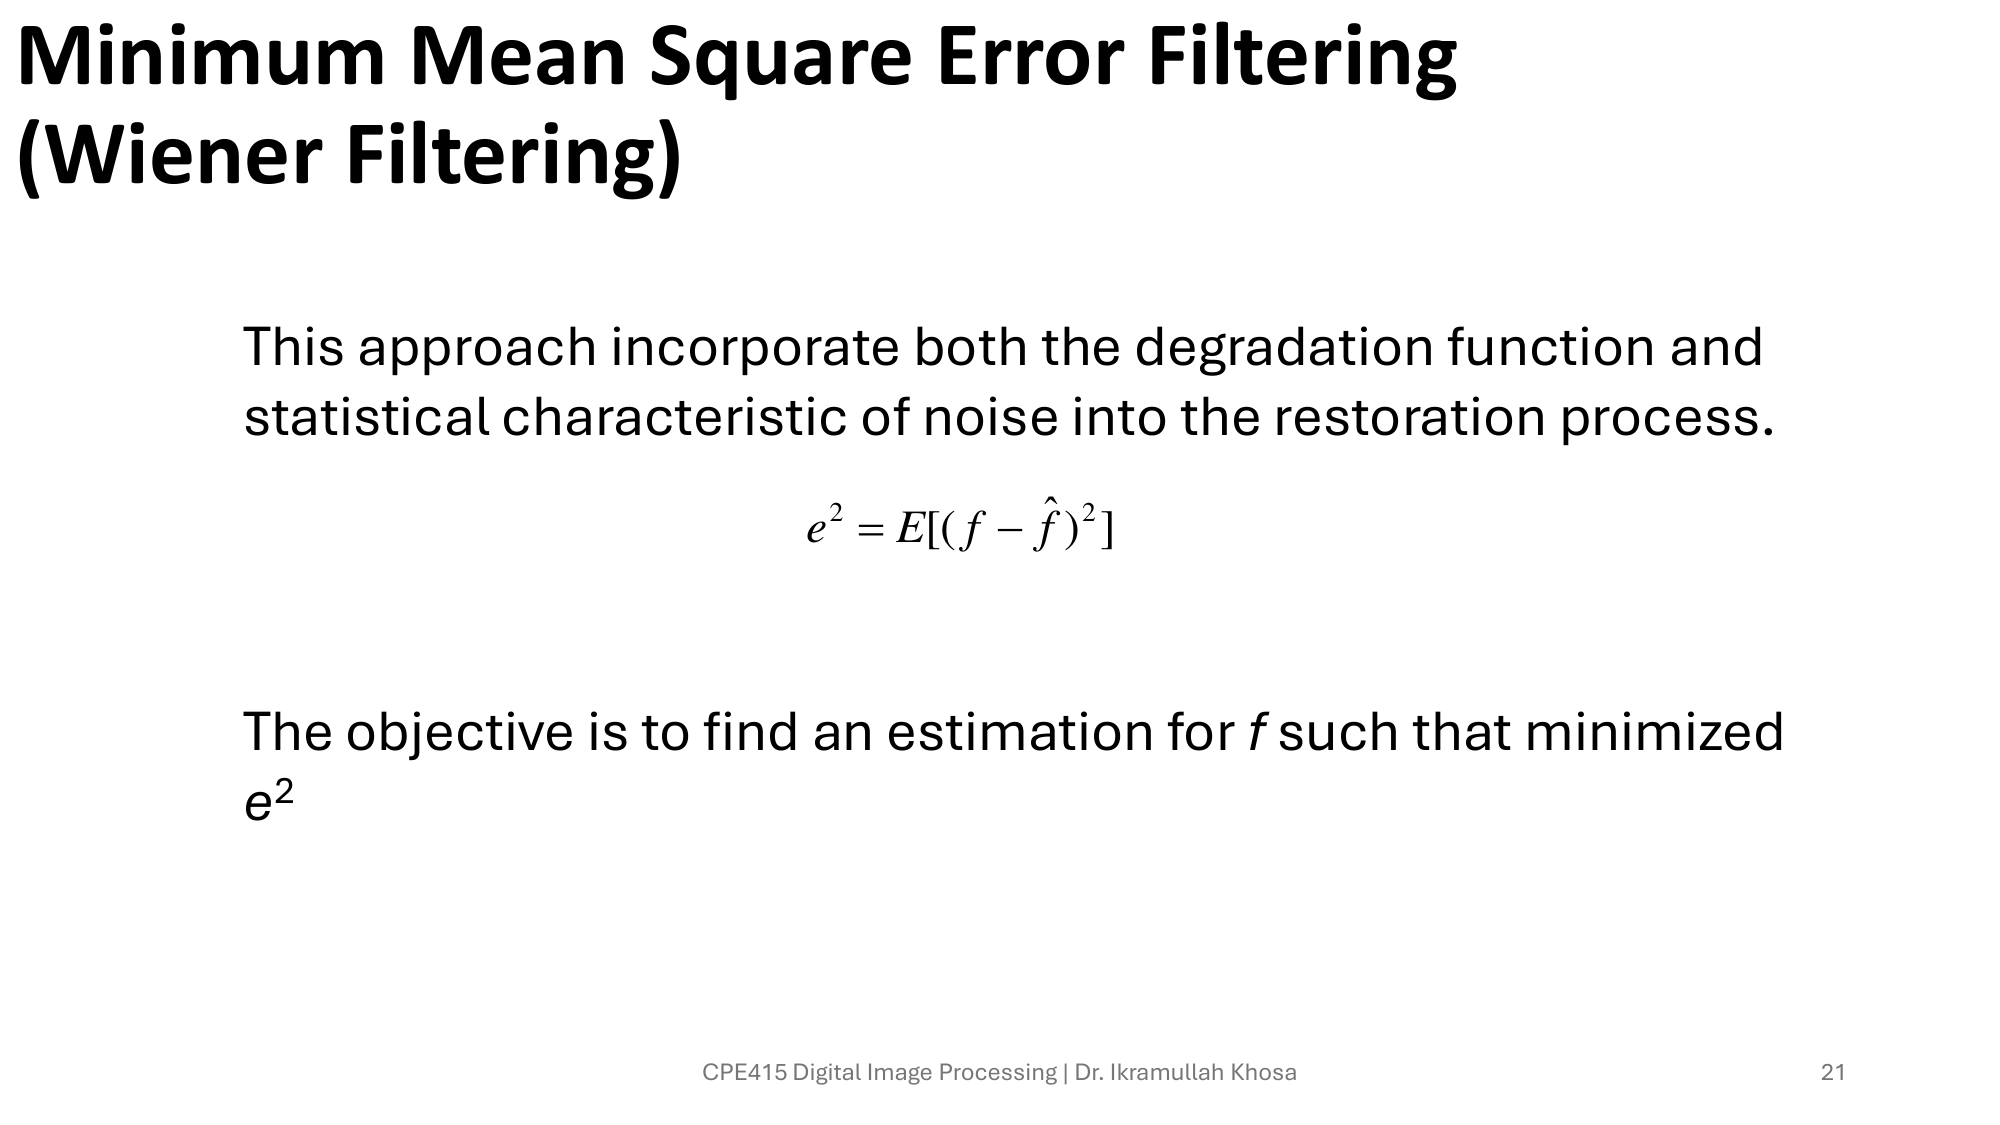
\includegraphics[width=0.85\textwidth]{images/slide12-21.png}
    \caption{MMSE objective used in Wiener filtering}
    \label{fig:wiener_mmse}
\end{figure}

\begin{figure}[H]
    \centering
    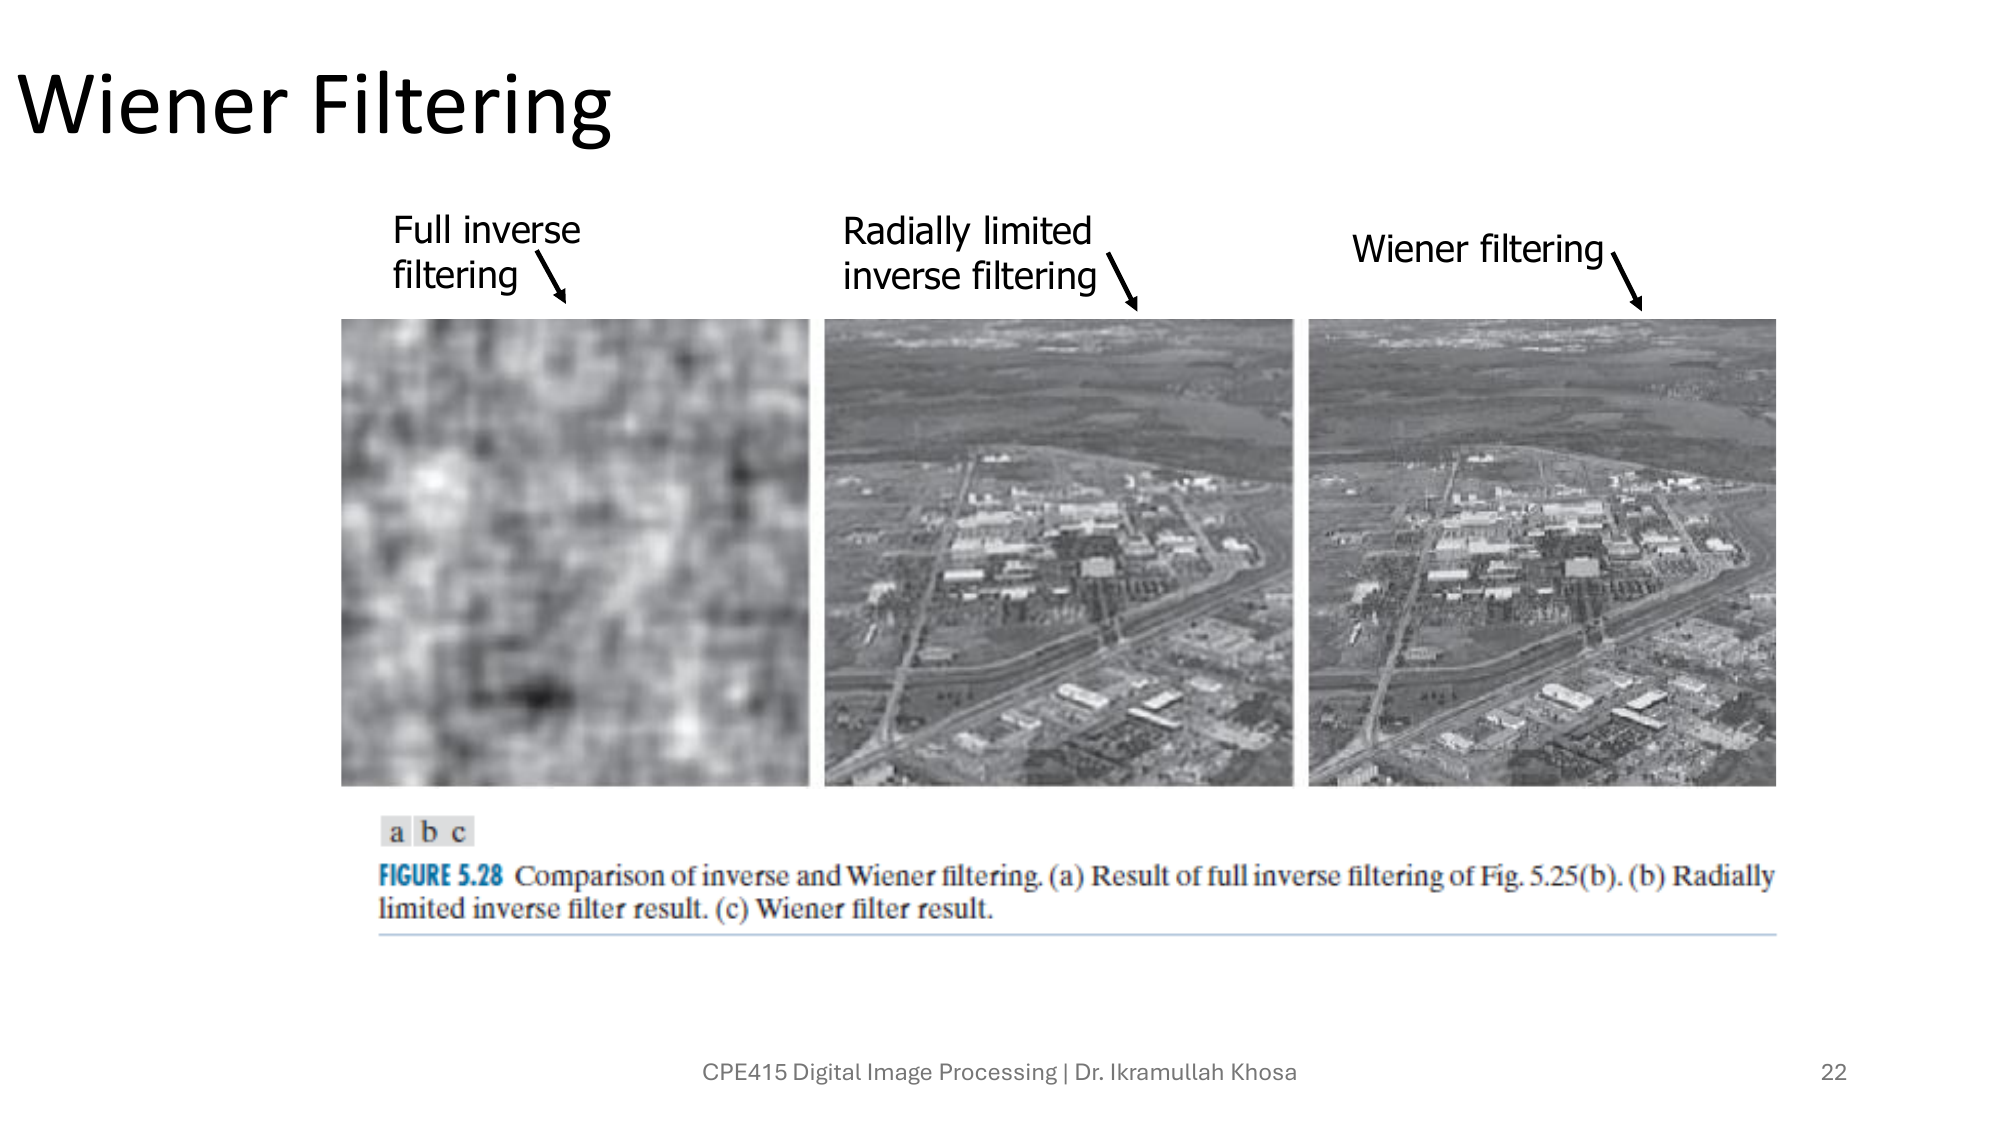
\includegraphics[width=0.9\textwidth]{images/slide12-22.png}
    \caption{Comparison: full inverse, radially limited inverse, Wiener filtering}
    \label{fig:wiener_compare1}
\end{figure}

\begin{figure}[H]
    \centering
    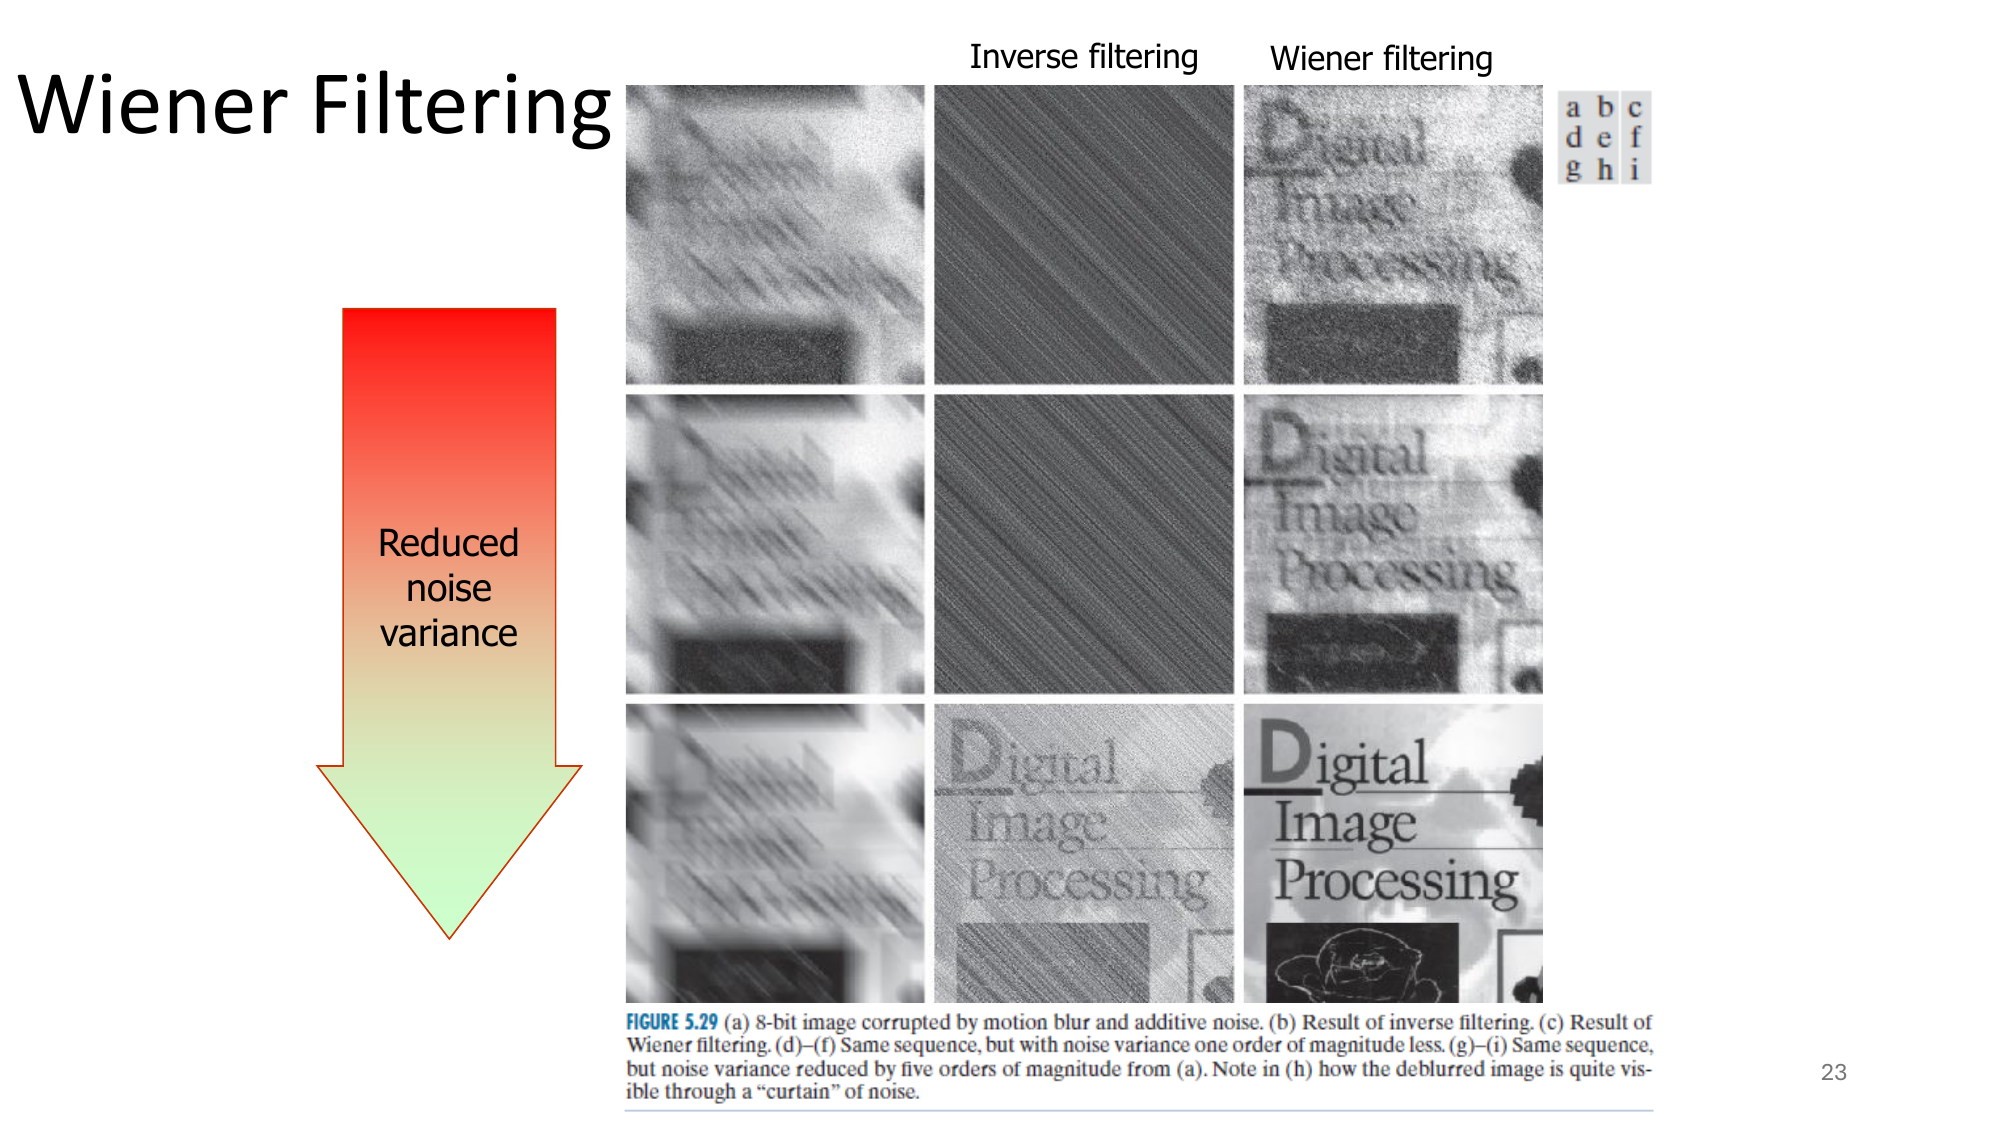
\includegraphics[width=0.9\textwidth]{images/slide12-23.png}
    \caption{Wiener filtering robustness under noisy conditions}
    \label{fig:wiener_compare2}
\end{figure}

\begin{deepexplanation}
\textbf{DEEP ANALYSIS: Why Wiener Beats Simple Inverse in Practice}

Inverse filter tries to undo blur exactly; Wiener filter performs \textbf{statistically optimal compromise}:
\begin{itemize}
    \item Deblur where signal dominates,
    \item suppress where noise dominates.
\end{itemize}

So Wiener filtering is not perfect deconvolution; it is minimum expected error estimation under stochastic assumptions.
\end{deepexplanation}

%==============================================================================
\section{Constrained Least Squares (CLS) Filtering}
%==============================================================================

CLS seeks a restored image that is smooth (via Laplacian penalty) while remaining consistent with observed data.

Frequency-domain form:
\[
\hat{F}(u,v)=\left[\frac{H^*(u,v)}{|H(u,v)|^2+\gamma|P(u,v)|^2}\right]G(u,v)
\]
where:
\begin{itemize}
    \item $\gamma$ controls regularization strength,
    \item $P(u,v)$ is FT of Laplacian operator
\end{itemize}

\[
p(x,y)=\begin{bmatrix}
0 & -1 & 0\\
-1 & 4 & -1\\
0 & -1 & 0
\end{bmatrix}
\]

\begin{conceptbox}[Wiener vs. CLS]
\textbf{Wiener:} needs degradation model plus spectral/statistical noise-image information.

\textbf{CLS:} can be implemented with weaker statistical assumptions; regularization controls noise amplification.

Both are significantly more stable than direct inverse filtering.
\end{conceptbox}

%==============================================================================
\section{Geometric Mean Filter}
%==============================================================================

A useful family that bridges inverse and Wiener behavior:
\[
\hat{F}(u,v)=\left[\frac{H^*(u,v)}{|H(u,v)|^2}\right]^\alpha
\left[\frac{H^*(u,v)}{|H(u,v)|^2+b\,S_\eta(u,v)/S_f(u,v)}\right]^{1-\alpha}
G(u,v)
\]
where $\alpha,b > 0$.

Special cases:
\begin{itemize}
    \item $\alpha=1$: inverse filter
    \item $\alpha=0$: parametric Wiener-type filter
    \item $\alpha=1/2$: geometric blend of both terms
\end{itemize}

%==============================================================================
\section{Practical Restoration Workflow (Exam-Friendly)}
%==============================================================================

\begin{enumerate}
    \item Identify degradation type (periodic noise, motion blur, turbulence, mixed).
    \item Build/estimate $H(u,v)$ using observation, experimentation, or modeling.
    \item If periodic spikes are visible, remove them first using notch reject filtering.
    \item Start restoration with Wiener or CLS (inverse only as baseline).
    \item Tune parameters ($K$, $\gamma$, notch width/radius) against artifact vs. detail tradeoff.
    \item Validate visually and, if possible, with MSE/SNR metrics.
\end{enumerate}

\begin{importantbox}
\textbf{Key exam takeaway:}
Image restoration is an inverse problem with noise-sensitive instability. All practical methods are different forms of \textbf{regularized inversion}.
\end{importantbox}

%==============================================================================
\section{Lecture 12: Critical Slide-by-Slide Explanation}
%==============================================================================

\subsection{Slide 1: Title Slide (Chapter 5)}
This slide sets scope, not content. Critically, it combines \textit{restoration} and \textit{reconstruction}, which are related but distinct: restoration starts from a degraded image, while reconstruction estimates an image from indirect measurements (for example projections in CT).

\subsection{Slide 2: Periodic Noise Reduction Overview}
This slide introduces the right toolbox (bandreject, bandpass, notch), but it is concept-dense and can confuse beginners. The key correction is that practical periodic-noise removal is usually notch-centered, because broad bandreject masks may remove too much real image detail.

\subsection{Slide 3: Periodic Noise Reduction (Visual Transition)}
This slide appears to be a transition visual without heavy formulas. Critically, transition slides should be read as workflow cues: identify spikes in spectrum, isolate them, then suppress selectively.

\subsection{Slide 4: Notch Pass vs Notch Reject Demonstration}
The side-by-side concept is important: notch-pass reveals what is being removed; notch-reject produces the cleaned result. The hidden risk is over-wide notches, which suppress neighboring legitimate frequencies and cause loss of texture.

\subsection{Slide 5: Repeated Notch Demonstration}
This repeat is pedagogically useful because notch design is empirical. Critical point: repeated examples imply parameter tuning is data-dependent; there is no single universal notch width or shape.

\subsection{Slide 6: Optimum Notch Filtering (Section Start)}
This is a heading slide introducing an optimization view. The critical shift is from binary filtering (keep/remove frequency) to adaptive subtraction with local statistical control.

\subsection{Slide 7: Ideal vs Estimated Noise Subtraction}
The slide correctly distinguishes $f=g-\eta$ (ideal) from $\hat{f}=g-\hat{\eta}$ (practical). Critical implication: all downstream methods are compensation methods for estimation error, not exact inversion methods.

\subsection{Slide 8: Modulation Function and Local Variance Objective}
Introducing $w(x,y)$ is the most important conceptual upgrade in notch filtering. Critically, local-variance minimization can suppress residual periodic interference, but it may also flatten fine local contrast if neighborhoods are too large.

\subsection{Slide 9: Constant-$w$ Neighborhood Assumption}
The assumption $w(x+s,y+t)=w(x,y)$ makes optimization tractable. The limitation is model bias: in highly nonstationary regions (edges/text), constant $w$ may be too coarse and can introduce local under/over-correction.

\subsection{Slide 10: Closed-Form Optimal $w(x,y)$}
The derived expression for $w$ is statistically meaningful (covariance/variance structure). Critical numerical caution: denominator values near zero can make $w$ unstable, so robust implementations clip or regularize.

\subsection{Slide 11: Block Diagram of Optimal Notch Filtering}
The block view clarifies pipeline order: estimate interference, compute modulation, subtract adaptively. Critical insight: errors in $\hat{\eta}$ propagate directly to output, so interference-estimation quality dominates final restoration quality.

\subsection{Slide 12: Optimum Notch Filtering Example Output}
This slide is mostly visual evidence. Critically, visual success must be judged for both objectives: reduced periodic pattern and preserved detail; often one improves at the expense of the other.

\subsection{Slide 13: Degradation Model and Estimation Routes}
This slide correctly frames the canonical model $g=H[f]+\eta$ and the three estimation routes. Critical exam point: restoration quality is bounded by the quality of $H$ estimation; even strong filters fail with poor model identification.

\subsection{Slide 14: Estimation by Image Observation}
The ratio $H_s=G_s/\hat{F}_s$ is intuitive but weakly grounded if $\hat{F}_s$ is unreliable. Critical weakness: this method is subjective and sensitive to region selection, so it is best for small, controlled corrections.

\subsection{Slide 15: Estimation by Experimentation}
Impulse-response estimation is the most physically grounded approach in controlled settings. Critical limitation: requires access to similar acquisition hardware and repeatable settings, which is often impractical in real-world restoration.

\subsection{Slide 16: Atmospheric Turbulence Modeling}
The model $H(u,v)=e^{-k(u^2+v^2)^{5/6}}$ is theoretically motivated and captures blur severity via $k$. Critical assumption: it implies isotropic, global behavior; real turbulence can be spatially varying and anisotropic.

\subsection{Slide 17: Motion Blur Derivation (Single-Axis Case)}
This slide links physical motion to a frequency-domain sinc-like response, which explains ringing and directional degradation. Critical takeaway: zeros in the motion transfer function make direct inversion highly sensitive.

\subsection{Slide 18: Motion Blur Derivation (General 2D Motion)}
Generalizing to both $a$ and $b$ makes the model realistic for oblique motion. Critical note: model validity depends on uniform velocity during exposure; acceleration or camera shake violates this assumption.

\subsection{Slide 19: Inverse Filtering and Its Instability}
The equation $\hat{F}=G/H$ is mathematically clean but practically fragile. Critical reason for failure is explicit in $\hat{F}=F+N/H$: when $|H|$ is small, noise amplification can dominate all restored content.

\subsection{Slide 20: Radius-Limited Inverse Filtering Results}
This slide demonstrates regularization by frequency truncation. Critical interpretation: this is a bias-variance tradeoff in frequency space; small radius leaves blur, large radius restores details but revives noise.

\subsection{Slide 21: MMSE Objective (Wiener Foundation)}
The objective $E[(f-\hat{f})^2]$ formalizes restoration as statistical estimation. Critical limitation: Wiener optimality depends on assumptions about second-order statistics and noise-image independence.

\subsection{Slide 22: Full Inverse vs Limited Inverse vs Wiener}
This comparison slide gives the practical verdict: Wiener usually outperforms naive inverse in noisy conditions. Critical nuance: "best" still depends on parameter estimation quality (for example $K$ or spectral ratios).

\subsection{Slide 23: Wiener Under Reduced Noise Variance}
This slide shows that as noise variance drops, restoration quality improves for both methods, but Wiener remains more stable. Critical conclusion: restoration is not only an algorithm problem; acquisition noise level fundamentally sets achievable quality.

%==============================================================================
\section{Quick Formula Sheet}
%==============================================================================

\begin{mathbox}
\textbf{Degradation model:}
\[
G=HF+N
\]

\textbf{Inverse filter:}
\[
\hat{F}=\frac{G}{H}
\]

\textbf{Wiener filter:}
\[
\hat{F}=\left[\frac{H^*}{|H|^2+S_\eta/S_f}\right]G
\]

\textbf{CLS filter:}
\[
\hat{F}=\left[\frac{H^*}{|H|^2+\gamma|P|^2}\right]G
\]

\textbf{Notch relation:}
\[
H_{NP}=1-H_{NR}
\]

\textbf{Motion blur model:}
\[
H(u,v)=\frac{T}{\pi(ua+vb)}\sin\left[\pi(ua+vb)\right]e^{-j\pi(ua+vb)}
\]
\end{mathbox}

\end{document}
